\documentclass[../main.tex]{subfiles}
\graphicspath{{\currfiledir}}
\begin{document}
\chapter{Terminology}

\section{Grapheme}
\textcquote[204]{crystal2010}{Graphemes are the smallest units in a writing system capable of 
causing a contrast in meaning.}
In linguistics, graphemes are often placed in angle brackets, e.g. \grapheme{a} or \grapheme{b}.
Sometimes \emph{graphemes} are called \emph{signs}.
The term \emph{sign} and \emph{grapheme} are considered to be equivalent and 
interchangeable throughout this work.

\section{Graph and allograph}
\textcquote[204]{crystal2010}{Graphemes are abstract units which may adopt a variety of forms 
\elide Each of these possible forms is known as \emph{graphs}\elide
There is a vast amount of physical variation in the shapes of graphs that does not affect the 
underlying identity of the grapheme\elide 
When graphs are analyzed as variants of a grapheme, they are known as \emph{allographs}.}
The Maya script uses a lot of allographs.
For example, the syllable \syllable{u} can be written in many ways all having the same meaning.
See~\ref{fig:terminology-grapheme-u-allographs} for a selection of allographs.
\begin{center}
    
\includegraphics[width=\textwidth,keepaspectratio]{img/grapheme-u-allographs}
    \captionof{figure}{Some allographs of the grapheme \grapheme{u}}
    \label{fig:terminology-grapheme-u-allographs}
\end{center}

\section{Hieroglyph and glyph}
The term \emph{hieroglyph} and \emph{glyph} are not precise terms.
Both are used in epigraphic literature, to address a group of one or more graphemes.
\textcquote[1]{bricker1986}{A ``glyph'' is a sign that can occur alone or in combination with 
other signs}.
\textcquote[34]{knorozov1967}{A hieroglyph consists of several graphemes, which are joined 
in writing}. 
Both expressions are considered to be equivalent and interchangeable throughout this work.
\emph{Glyphs} can represent a syllable, a single word or even a whole phrase 
(\cite[23]{macrilooper2003}).

For example, the glyph~\ref{fig:terminology-glyphs-utzapaw} consists of the 
graphemes \grapheme{u}, \grapheme{tz\glottalstop{}a} and \grapheme{wa} representing the phrase
\mayan{u tz\glottalstop{}apaw}, ``she/he erects it''.
% LTeX: enabled=false
The glyph~\ref{fig:terminology-glyphs-ixwinikhaabajaw} consisting of the 
graphemes \grapheme{ix}, \grapheme{winikhaab} and \grapheme{ajaw}
and represents the noble title \mayan{ix winikhaab ajaw}, ``Ruler Lady Winikhaab''.
\begin{figure}
    \centering
    \begin{subfigure}[b]{0.49\textwidth}
        \centering
        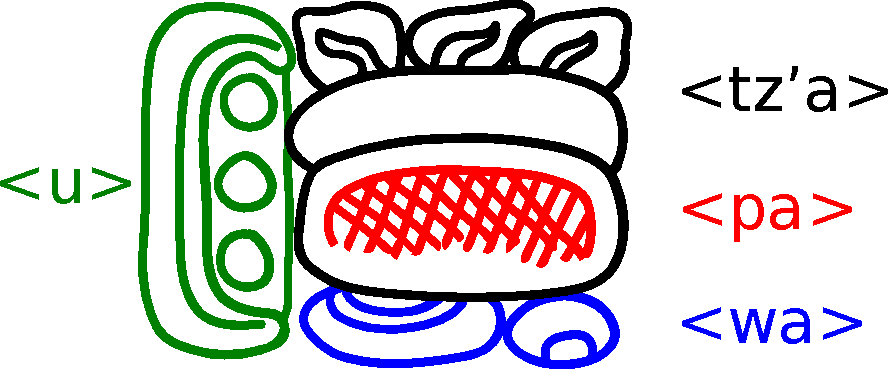
\includegraphics[height=\glyphblockheight]{img/glyphs-utzapaw}
        \caption{\mayan{u tz\glottalstop{}apaw}}
        \label{fig:terminology-glyphs-utzapaw}
    \end{subfigure}
    \hfill
    \begin{subfigure}[b]{0.49\textwidth}
        \centering
        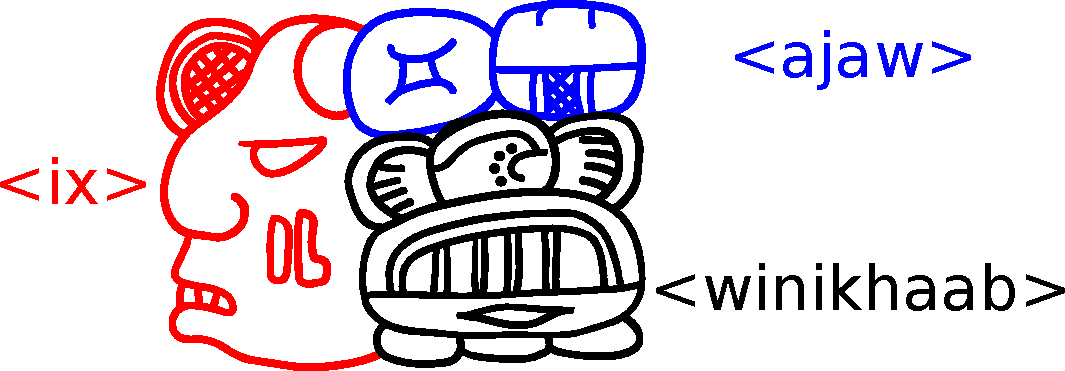
\includegraphics[height=\glyphblockheight]{img/glyphs-ixwinikhaabajaw}
        \caption{\mayan{ix winikhaab ajaw}}
        \label{fig:terminology-glyphs-ixwinikhaabajaw}
    \end{subfigure}
    \caption{Sample glyphs: graphemes are distinguished by different colors}
\end{figure}
% LTeX: enabled=true

\section{Glyph block and collocation}
One or more \emph{Glyphs} are usually arranged in regular rectangular shapes called a 
\emph{glyph block}.
Sometimes they are also called \emph{collocation}.
\textcquote[1]{bricker1986}{A ``collocation'' is a group of signs that occupies a 
defined space, or block, in a hieroglyphic text.}
\textcquote[23]{macrilooper2003}{The rectangular shape of \emph{glyph blocks} results from 
the arrangement of texts into rows and columns}.
\todo{Image/drawing which shows rows and columns of glyphs}

\section{Theory in decipherment}
\textcquote[2]{zender2017}{The type of writing system must be known}.

\subsection{Script typology}
For successful decipherment process, it is crucial to know the fundamental structure of the signs.
The type of the script can either be alphabetic, syllabic, logographic or a combination of them.
In order to classify an unknown writing system, the number of signs employed in the scripts
can hint what type of writing system one deals with.
% LTeX: enabled=false
Johannes Friedrich observed:
\blockquote[{\cite[152]{friedrich1957}}]{\elide~the number of the written symbols usually warrants a 
conclusion as to whether the script is alphabetic, a pure syllabary (as in the Cypriote) or a
mixture of ideographic word-signs and syllabic signs (like the cuneiform writing or the Hittite
hieroglyphic script). A script consisting of less than thirty signs will presumably turn out to
be alphabetic\elide~Scripts containing fifty, a hundred or even several hundred different symbols
may justifiably be regarded beforehand as more or less complicated syllabic systems of writing,
perhaps employing also word-signs\elide}.
% LTeX: enabled=true
Based on Ignace Gelb (\cite[115]{gelb1963}), Michael Coe (\cite[43]{coe1992}) compiled a list
of writing systems and compared their type with the number of distinct signs
(see~\ref{table:terminology-writing-systems-comparison}).
\begin{table}[!ht]
    \centering
    \begin{tabular}{llc}
        \textbf{Type}                                                     & \textbf{Writing system} & \textbf{\# of signs} \\
        \multirow[t]{4}{20em}{\textbf{Logographic and Logosyllabic}\\
        Assigns a morpheme/word to each grapheme\\
        Logograms are either used for their semantic of syllabic values}  & Sumerian                & 600+ \\
                                                                          & Egyptian                & 2500 \\
                                                                          & Hittite Hieroglyphic    & 497 \\
                                                                          & Chinese                 & 5000+ \\
        \\
        \multirow[t]{4}{20em}{\textbf{Syllabic}\\
        Assigns a syllable to each grapheme}                              & Persian                 & 40 \\
                                                                          & Linear B                & 87 \\
                                                                          & Cypriot                 & 56 \\
                                                                          & Cherokee                & 85 \\
        \\
        \multirow[t]{3}{20em}{\textbf{(Augmented) Abjad}\\
        Assigns a consonant to each grapheme\\
        In augmented abjad some voxels are added} \\
                                                                          & Phoenician              & 22 \\
                                                                          & Ugaritic                & 30 \\
        \\                                                                 
        \multirow[t]{7}{20em}{\textbf{(Augmented) Alphabet}\\
        Assigns a vowel or consonant to each grapheme}                    & English                 & 26 \\
                                                                          & Anglo-Saxon             & 31 \\
                                                                          & Sanskrit                & 35 \\
                                                                          & Etruscan                & 20 \\
                                                                          & Russian                 & 36 \\
                                                                          & Hebrew                  & 22 \\
                                                                          & Arabic                  & 28 \\
    \end{tabular}
    \caption{Writing systems, their types and their number of distinct signs 
             (after~\cite[43]{coe1992},~\cite[730]{daniels1990},~\cite[88]{coulmas1991}
             and~\cite{ritner1996})}
    \label{table:terminology-writing-systems-comparison}
\end{table}


Michael Coe missed several mixed writing systems

\subsection{Corpus}

\subsection{Language}

\subsection{Cultural context}

\subsection{Bilingual, biscript, or similar constraint}


\section{Cataloging of signs}
One of the first steps to analyze an unknown writing system, is to identify distinctive graphemes 
and their allographs. 
In the past, several sign catalogs have been proposed.
Yuri Knorozov created a sign catalog in his work (\cite[109\psq]{knorozov1967}).
William E. Gates' and G\"unter Zimmermann's catalogs (\cite{gates1931},~\cite{zimmermann1956}) are 
based on the Maya codices but did not include the signs from the inscriptions 
(\cite[4]{thompson1962catalog}). 
Eric Thompson extended G\"unter Zimmermann's idea and categorized all signs into affixes, main signs 
(including animal heads) and portrait signs (\cite[4]{thompson1962catalog}).
His catalog covers the Maya codices, the monumental inscriptions and other writings 
(e.g.\ ceramics, vessels, bones).
All catalogs assigned a number to each sign/grapheme.
To distinguish between the different catalog systems, it is common to use a prefix in 
conjunction with the number.
So, for example, all Thompson numbers are labeled with the prefix ``T'', e.g. \thompson{510}.

In 2003, Martha J. Macri and Matthew G. Looper proposed a new system which assigns all graphemes
a code consisting of three digits (\cite[21,25]{macrilooper2003}).
The first two digits specifies the category of the sign 
(e.g. A for animals, M for signs with hands etc.) whereas the third digit is an arbitrary number
sequencing the different graphemes.

The project ``Text Database and Dictionary of Classic Mayan'' (abbr. TWKM) (\cite{twkm2014}) lead by 
Prof.\ Dr.\ Nikolai Grube of the Department of Anthropology of the Americas at the University of 
Bonn is currently compiling an updated and revisited version of Thompson's sign catalog.
% LTeX: enabled=false
Christian Prager states, \textcquote{prager2020}{we are currently evaluating and revising Eric 
Thompson’s Catalog of Maya Hieroglyphs (1962). 
We are critically scrutinizing his system with the help of his original grey cards and 
supplementing it with signs that were not included in Thompson’s original catalogue. 
Despite its known shortcomings and incompleteness, his catalogue is still regarded as the 
standard work for Maya epigraphers, which is why we adopt Thompson’s nomenclature while 
removing misclassifications and duplicates, merging graph variants under a common nomenclature, 
and adding new signs or allographs to the sign index in sequence, starting with the number 1500.
}
% LTeX: enabled=true

\subsection{Problems and limitations}
Having all these sign catalogs are a huge help to systematically analyze any writing system.
It is especially important when the writing system cannot be read.
As one could see above, researchers assign codes or numbers to address individual or 
even groups of signs.
Therefore, identifying graphemes are crucial to systematically build up a sign catalog.
Yet, determine them in an unknown writing system is challenging.
One way to approach this, is by segmenting the texts into distinct \emph{graphs}.
Researchers hereby followed the assumption that graphemes of a script are considered the same if 
they resemble each other in more features than either resembles any other.
\textcquote[34]{knorozov1967}{Two [signs] are identical when they are both composed of the same 
graphic elements\elide, whose drawing and disposition is sufficiently similar to allow them to 
be identified}.
However, if there is no control in terms of linguistics and content, 
this approach can be problematic.
Three major issues can occur when segmenting signs from an unknown writing system.
\begin{itemize}
    \item Allographs are interpreted as separate graphemes.
    \item Graphemes with distinct phonemes and meanings are interpreted as allographs.
    \item Complex graphemes are split into its sub-graphemic components.
\end{itemize}
Especially in writing systems with many allographs like the Maya hieroglyphs,
allographs are sometimes not recognized and, instead, are interpreted as separate graphemes. 
Sometimes, signs are considered to be allographs because of their similarities, 
but, as later progress in decipherment has shown, were actually distinct graphemes.
Eric Thompson (\cite[12\psq]{thompson1962catalog}) recognized the method of segmentation as 
a potential source of false conclusions.
David Kelley (\cite{kelley1962}) was able to show in his review of Thompson's sign catalog that
some T-numbers represent more than one grapheme 
(e.g. \thompson{683a} and \thompson{T683b}~\ref{fig:terminology-t683a-t683b}) 
and some T-numbers are allographs of another 
(e.g. \thompson{589} and \thompson{T607}~\ref{fig:terminology-t589-t607}).
% LTeX: enabled=false
\begin{figure}
    \centering
    \begin{subfigure}[b]{0.49\textwidth}
        \centering
        
\includegraphics[height=\glyphblockheight]{img/T683a-T683b}
        \caption{\grapheme{winik} and \grapheme{ja} assigned to \thompson{683}}
        \label{fig:terminology-t683a-t683b}
    \end{subfigure}
    \hfill
    \begin{subfigure}[b]{0.49\textwidth}
        \centering
        
\includegraphics[height=\glyphblockheight]{img/T589-T607}
        \caption{\grapheme{ho} assigned to \thompson{589} and \thompson{607}}
        \label{fig:terminology-t589-t607}
    \end{subfigure}
    \caption{Wrong T-number assignment in Thompson's catalog (after Kelley)}
\end{figure}
% LTeX: enabled=true
Despite merging unrelated graphs or separating allographs which actually belong to each other,
the Maya writing system also utilizes graphemes which consist of two or more subgraphemic 
components.
Those complex graphemes might not be recognized and therefore only its components are registered
as graphemes.
One of those complex graphemes, is the grapheme \grapheme{pas} ``dawn'' 
(\ref{fig:terminology-glyphs-pas}) which is built from
grapheme \grapheme{chan} ``sky'' (\ref{fig:terminology-glyphs-chan}), 
grapheme \grapheme{k\glottalstop} ``k\glottalstop{}in'' (\ref{fig:terminology-glyphs-kin}) and
grapheme \grapheme{kab} ``earth'' (\ref{fig:terminology-glyphs-kab}).
It can be found, for example, on Tikal Temple IV, Lintel 2 A7.
All three components are graphemes themselves, but in combination they form the complex 
grapheme \grapheme{pas} with its phoneme and meaning.
This grapheme doesn't show up in Thompson's sign catalog.
Later revisions and new catalogs like Macri and Looper (\cite{macrilooper2003}) added it as
separate grapheme and assigned it the code ZX2.
% LTeX: enabled=false
\begin{figure}
    \centering
    \begin{subfigure}[b]{0.24\textwidth}
        \centering
        
\includegraphics[height=\glyphblockheight]{img/grapheme-PAS}
        \caption{\grapheme{pas} ``dawn''}
        \label{fig:terminology-glyphs-pas}
    \end{subfigure}
    \hfill
    \begin{subfigure}[b]{0.24\textwidth}
        \centering
        
\includegraphics[height=\glyphblockheight]{img/grapheme-CHAN}
        \caption{\grapheme{chan} ``sky''}
        \label{fig:terminology-glyphs-chan}
    \end{subfigure}
    \begin{subfigure}[b]{0.24\textwidth}
        \centering
        
\includegraphics[height=\glyphblockheight]{img/grapheme-KIN}
        \caption{\grapheme{k\glottalstop{}in} ``sun''}
        \label{fig:terminology-glyphs-kin}
    \end{subfigure}
    \begin{subfigure}[b]{0.24\textwidth}
        \centering
        
\includegraphics[height=\glyphblockheight]{img/grapheme-KAB}
        \caption{\grapheme{kab} ``earth''}
        \label{fig:terminology-glyphs-kab}
    \end{subfigure}
    \caption{Grapheme \grapheme{pas}. Even though it consists of three other graphemes, 
             it represents a self-contained grapheme with separate phonetic and meaning 
             (\cite[139]{prager2018}).}
\end{figure}
% LTeX: enabled=true

\end{document}
